% Gemini theme
% https://github.com/anishathalye/gemini

\documentclass[final]{beamer}

% ====================
% Packages
% ====================

\usepackage[T1]{fontenc}
\usepackage{lmodern}
\usepackage[size=custom,width=83.82,height=60.96,scale=1.0]{beamerposter}
\usetheme{gemini} %\usecolortheme{gemini}
\usecolortheme{owl}
\usepackage{graphicx}
\usepackage{booktabs}
\usepackage{tikz}
\usepackage{amssymb}
\usepackage{amsmath}
\usepackage{pgfplots}
\usepackage{tabularx}
\usepackage{enumitem}
\usepackage{caption,amsmath,graphicx,url,amssymb,latexsym,epsfig,tabularx,setspace,multirow,threeparttable,longtable,pdflscape,tabu,comment,subfigure,textcomp,xparse}

\definecolor{darkblue}{RGB}{39, 60, 200}
\setbeamercolor{headline}{fg=lightgray,bg=darkblue}
\setbeamercolor{headline rule}{bg=darkblue}


% ====================
% Lengths
% ====================

% If you have N columns, choose \sepwidth and \colwidth such that
% (N+1)*\sepwidth + N*\colwidth = \paperwidth
\newlength{\sepwidth}
\newlength{\colwidth}
\setlength{\sepwidth}{0.010\paperwidth}
\setlength{\colwidth}{0.3\paperwidth}

\newcommand{\separatorcolumn}{\begin{column}{\sepwidth}\end{column}}

% ====================
% Control Sequences
% ====================

%\def\DtoH{\textit{DtoH}\xspace}
%\def\HtoD{\textit{HtoD}\xspace}

\def\DtoH{\textit{DtoH}}
\def\HtoD{\textit{HtoD}}

% ====================
% Title
% ====================

\title{The Acceleration of Algorithms With Low Compute to Memory Access Ratios on Heterogeneous CPU/GPU Platforms}

\author{Zane Fink\inst{1}, Jordan Wright\inst{1}, and Michael Gowanlock\inst{1}}

\institute[shortinst]{\inst{1} School of Informatics, Computing, and Cyber Systems at Northern Arizona University}

% ====================
% Body
% ====================

\begin{document}

\begin{frame}[t]
\begin{columns}[t]
\separatorcolumn

\begin{column}{\colwidth}

  \begin{block}{Abstract}

   %Many operations common in high performance computing applications have a low compute to memory access ratio where achieving performance gains is perceived as insurmountable.
   %We examine several of these memory-bound algorithms, 
   %including $(i)$ linear scan; $(ii)$ batched predecessor searches; and, $(iii)$ multiway merging. 
   %For each, we examine the performance of parallel CPU-only, GPU-only, and hybrid CPU/GPU approaches, and show 
   %that hybrid algorithms achieve performance gains. We develop a model that considers 
   %main memory accesses and PCIe data transfers, which are two major bottlenecks for hybrid CPU/GPU algorithms. 
   %The model lets us determine how to share work between the CPU and GPU to maximize resource 
   %utilization while minimizing load imbalance. We show that our model can accurately predict the fraction of work 
   %to be sent to each, and thus confirms that these overlooked operations can be 
   %accelerated. 

   Many operations common in high performance computing applications have a low compute to memory access ratio where achieving performance gains is perceived as insurmountable.
   We examine several of these memory-bound algorithms, 
   including $(i)$ linear scan; $(ii)$ batched predecessor searches; and, $(iii)$ multiway merging. 
   For each, we examine the performance of parallel CPU-only, GPU-only, and hybrid CPU/GPU approaches, and show 
   that hybrid algorithms achieve performance gains. We develop a model that considers 
   main memory accesses and PCIe data transfers. The model lets us determine how to share work between the CPU and GPU to maximize resource 
   utilization while minimizing load imbalance. We show that our model can accurately predict the fraction of work 
   to be sent to each, and thus confirms that these overlooked operations can be 
   accelerated. 
  \end{block}

  \begin{block}{Introduction}
    
\begin{description}[font=$\bullet$~\normalfont\scshape\color{red!50!black}]

\item While compute-intensive operations have seen performance gains using GPUs, memory-bound algorithms often do not exploit the GPU.

\item One approach to improve the performance of memory-bound algorithms is to develop hybrid parallel algorithms that use both CPU and GPU resources.

%\item We utilize both the CPU and GPU to compute these HPC primitives.

\item We propose \emph{accelerating the unacceleratable} --- which we define as memory-bound algorithms that are well-suited to a hybrid CPU/GPU execution but not necessarily a GPU-only execution. 

%\item Our model for both CPU and GPU performance uses the well-known external memory (EM) model with the exception that we consider the total number of main memory \emph{elements} loaded/stored as our performance metric.

\end{description}  

  \end{block}

  %\begin{alertblock}{Problem Statement}
  % For each of our studied algorithms we implement CPU-only, GPU-only, and hybrid CPU/GPU algorithms. 
  % We consider a platform with multi-core CPUs and a GPU, where the total response time includes all 
  % data transfers to and from the GPU and related overheads. We assume that each algorithm can exceed the GPU's global memory capacity. 
  % We evaluate our model on two criteria: fraction load imbalance and speedup of the hybrid algorithms over CPU-only and GPU-only algorithms.
  %\end{alertblock}
\begin{alertblock}{Microbenchmarks}
 
\begin{description}[font=$\bullet$~\normalfont\scshape\color{red!50!black}]

\item Let $\beta$ be the unidirectional bandwidth over PCIe, $\gamma$ be the memory bandwidth between the CPU and main memory when reading, and $\alpha$ be the memory bandwidth between the CPU and main memory when simultaneously reading and writing. On our platform: $\alpha=19.56$~GiB/s, $\gamma=34.01$~GiB/s, and $\beta=11$~GiB/s.

\item Our platform contains 2$\times$ Intel Xeon E5-2620 v4 processors, 16 physical cores, at a clock rate of 2.1 GHz, and 128 GiB of main memory, equipped with a Quadro GP100 with 16 GiB of global memory.

\end{description} 
\begin{figure}[htp]
\centering
%width=0.22
    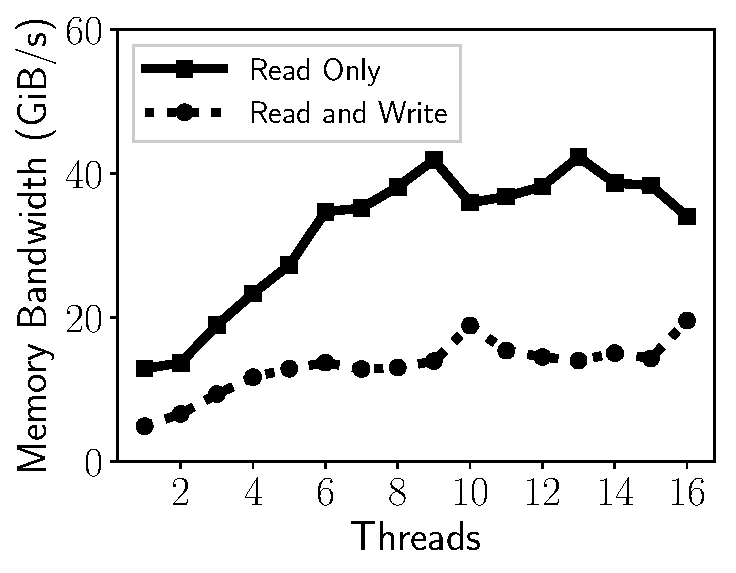
\includegraphics[height=0.25\textwidth, width=0.45\textwidth, trim={0.5cm 0.5cm 0.5cm 1cm}]{figures/microbenchmarks_time_vs_threads.pdf}	
    %\caption{Main memory bandwidth vs. the number of threads. Multiple threads are needed to saturate memory bandwidth. Simultaneous reading and writing has lower throughput than reading only.}
   \label{fig:mem_bandwidth_scalability}
\end{figure}

%\begin{description}[font=$\bullet$~\normalfont\scshape\color{red!50!black}]

%\end{description} 

\end{alertblock}


\end{column}

\separatorcolumn

\begin{column}{\colwidth}




 \begin{block}{Hybrid Algorithms}

 \begin{description}[font=$\bullet$~\normalfont\scshape\color{red!50!black}]
\item The three algorithms that we consider are parallelizable across both architectures while minimizing memory accesses. 
%We accomplish this by breaking up the total work into several \emph{batches} of divisible workloads that can be computed independently on either architecture. 

%\item We model evenly splitting the workloads based on PCIe and memory bandwidth to obtain low load imbalance (i.e., architectures finish computing their respective queries at similar times).

%\item We define $n_b$ to be the number of batches. For batched predecessor search and scan, we arbitrarily select $n_b=400$, while for multiway merge, we make $n_b$ a function of $k$, where $n_b=\frac{3200}{k}$. 

\item To model evenly splitting the work between architectures, let $f$ be the fraction of $n$ elements computed on the CPU, where $1-f$ is the fraction of $n$ computed on the GPU.

\item The total time to execute the CPU- and GPU-only algorithms are denoted as $T^{CPU}$ and $T^{GPU}$, respectively,
  which we estimate to be the number of elements accessed in memory for CPU divided by $\gamma$ for the scan,
  and $\alpha$ for the merge; and the number of elements accessed in memory for GPU divided by $\beta$.

\end{description}

\heading{Scan}
The scan algorithm examines every algorithm in a list (e.g. to find the maximum element).
We compute $f$ as a function of the parameters $\gamma$ and $\beta$, and set $T^{CPU}=T^{GPU}$. Therefore,
\begin{equation}f=\frac{\gamma}{\gamma+\beta}.\label{eqn:scan_split}\end{equation}


\heading{Batched Predecessor Search}
   For the predecessor search, we consider two sorted lists, $A$ and $B$. For each element of $B$, we wish to find the largest element of $A$
   less than that element of $B$.
   As before, $f$ is computed as,
\begin{equation}f=\frac{2\alpha}{2\alpha+3\beta}.\label{eqn:batch_predecessor_split}\end{equation}

\heading{Multiway Merging}
The multiway merge merges some number ($k$) of sorted sublists into one large sorted list.
Similarly to the scan, $f$ is computed as,
\begin{equation}f=\alpha/(\alpha+2\beta)\label{eqn:multiway_split}.\end{equation}

  \end{block}

\begin{block}{Research Highlights}
\begin{figure}[htp]
\centering
\subfigure[]{
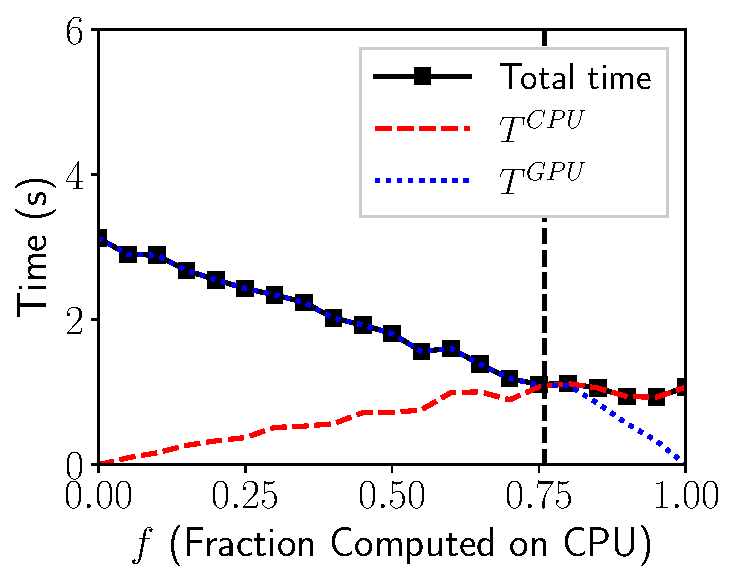
\includegraphics[height=0.26\textwidth, width=0.3\textwidth, trim={0.2cm 0.2cm 0.2cm 0.2cm}]{figures/time_vs_cpu_frac_scan.pdf}
}
\subfigure[]{
    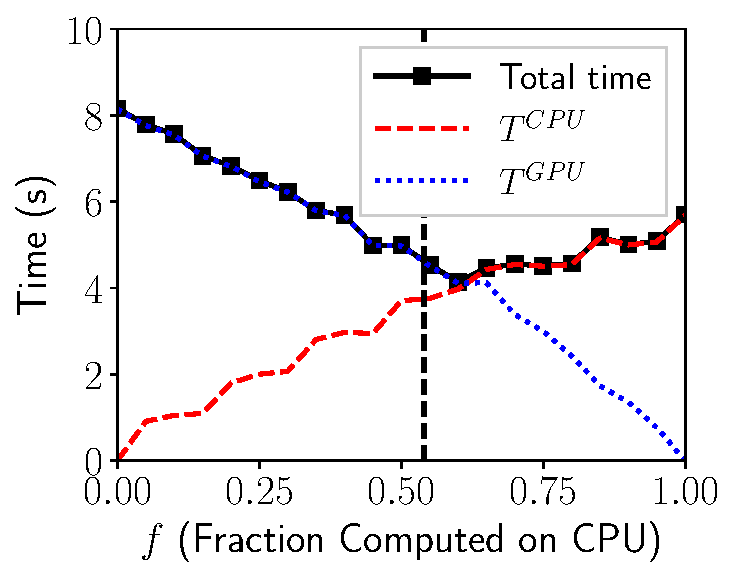
\includegraphics[height=0.26\textwidth, width=0.3\textwidth, trim={0.2cm 0.2cm 0.2cm 0.2cm}]{figures/time_vs_cpu_frac_predecessor.pdf}     
    }
\subfigure[]{
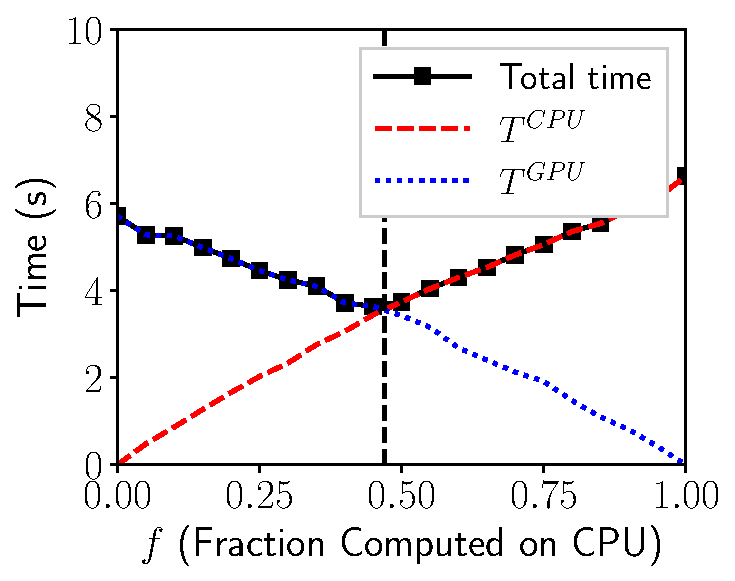
\includegraphics[height=0.26\textwidth, width=0.3\textwidth, trim={0.2cm 0.2cm 0.2cm 0.2cm}]{figures/time_vs_cpu_frac_multiway.pdf}}

%\captionsetup[figure]{font=small}
 \caption{Hybrid model accuracy for the scan, batched predecessor search, and multiway merging. The total response time, $T^{CPU}$, and $T^{GPU}$ vs. $f$, are plotted. We show $n=4.0\times10^9$ for all algorithms. The vertical dashed line in each plot denotes the modeled value of $f$.}

 \label{fig:time_vs_f}
\end{figure}

\end{block}

\end{column}

\separatorcolumn

\begin{column}{\colwidth}

  \begin{block}{Research Highlights (Cont.)}

%\begin{description}[font=$\bullet$~\normalfont\scshape\color{red!50!black}]
%\item Figure 2(a) demonstrates that the model accurately predicts $f$ for the scan ($f=0.76$).
%\item  Figure2(b) indicates that the model's prediction is quite accurate for multiway merging ($f=0.47$).
%\item  Figure 2(c) shows that even if the model can predict a good value for $f$ for batched predecessor search, small differences in $f$ can yield significant load imbalance ($f=0.35$). 
%\end{description}

%trim={0.2cm 0.2cm 0.2cm 0.2cm}
\begin{figure}[htp]
\centering
\subfigure[]{
    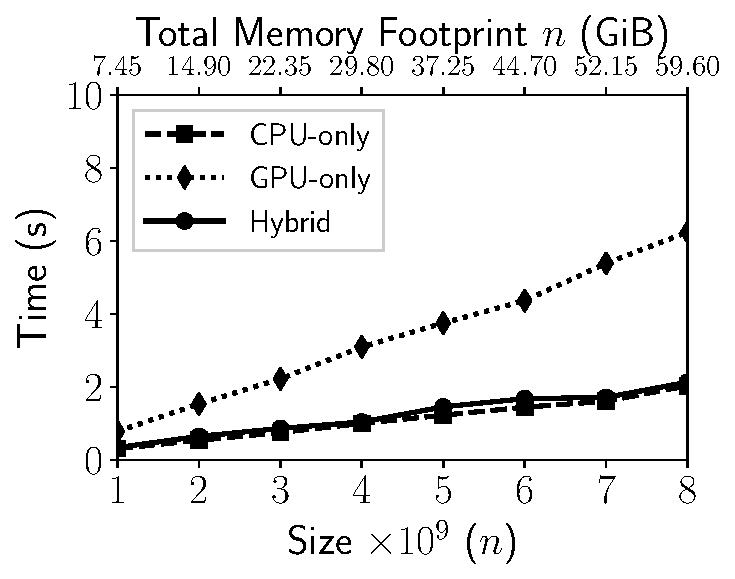
\includegraphics[height = 0.27\textwidth, width=0.30\textwidth, trim={0.2cm 0.2cm 0.2cm 0.2cm}]{figures/size_vs_time_linear_scan.pdf}	
}
\subfigure[]{
    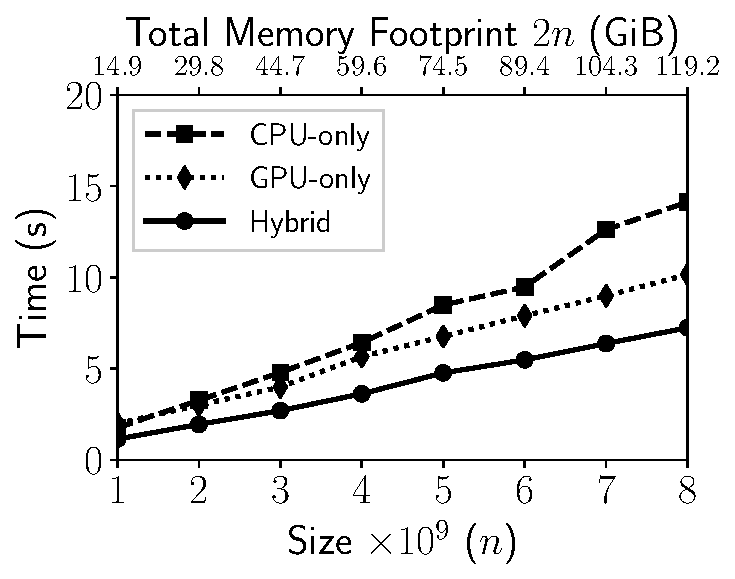
\includegraphics[height=0.27\textwidth, width=0.30\textwidth, trim={0.2cm 0.2cm 0.2cm 0.2cm}]{figures/size_vs_time_multiway.pdf}	
}
\subfigure[]{
    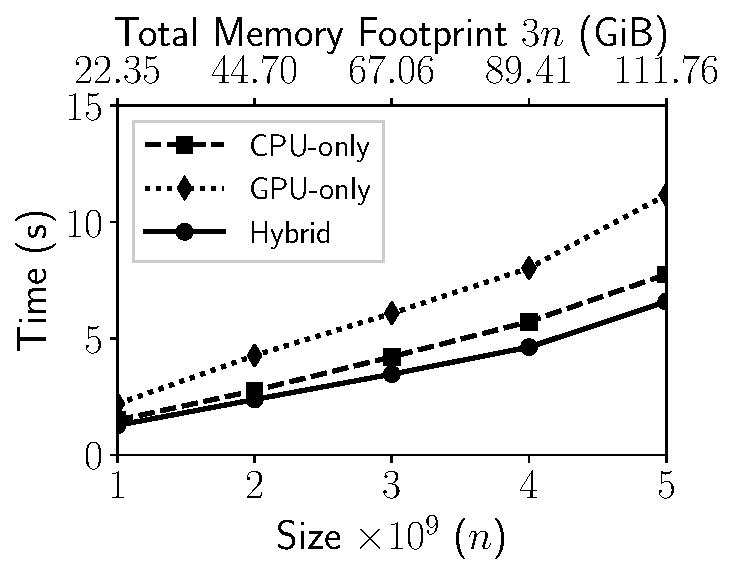
\includegraphics[height=0.27\textwidth, width=0.30\textwidth, trim={0.2cm 0.2cm 0.2cm 0.2cm}]{figures/size_vs_time_predecessor.pdf}	
}
   \caption{CPU-Only, GPU-Only and Hybrid runtimes for the scan (a), multiway merging (b), and batched predecessor search (c).}
   \label{fig:predecessor_search_results}
\end{figure}


\begin{figure}[t]
\centering
\subfigure[]{
    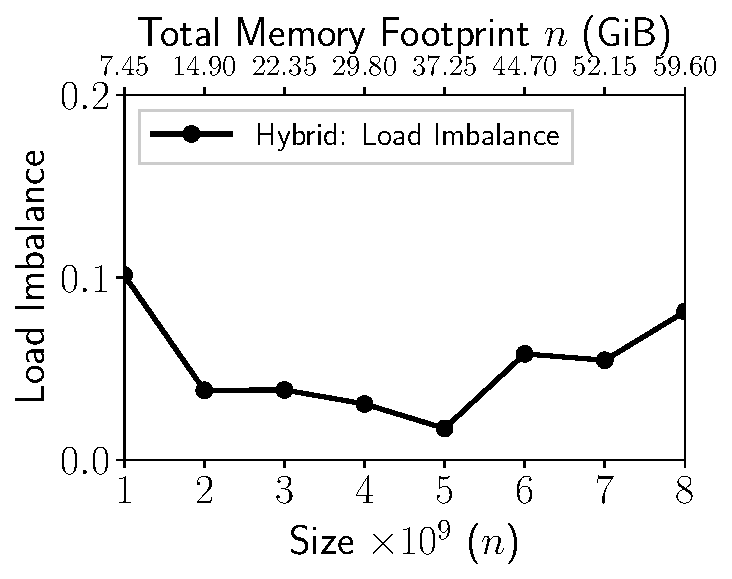
\includegraphics[height = 0.27\textwidth, width=0.30\textwidth, trim={0.2cm 0.2cm 0.2cm 0.2cm}]{figures/size_vs_load_imbalance_ls.pdf}	
    }
\subfigure[]{
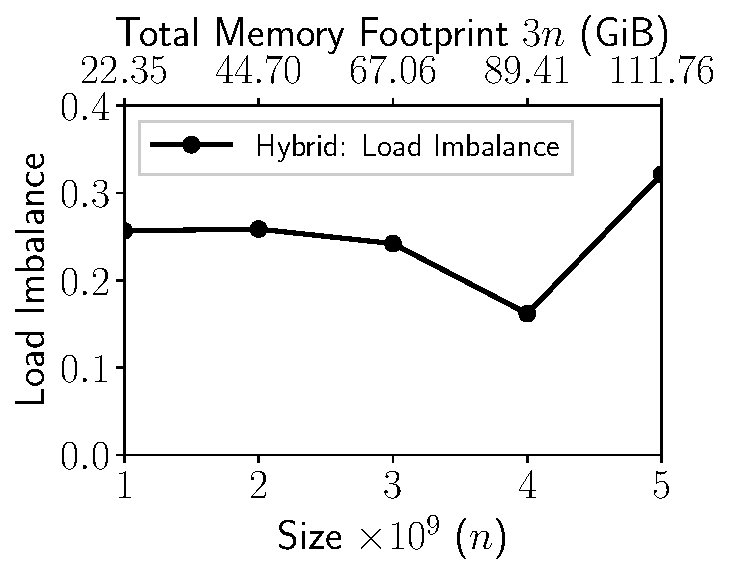
\includegraphics[height = 0.27\textwidth, width=0.30\textwidth, trim={0.2cm 0.2cm 0.2cm 0.2cm}]{figures/size_vs_load_imbalance_predecessor.pdf}	
    }
\subfigure[]{
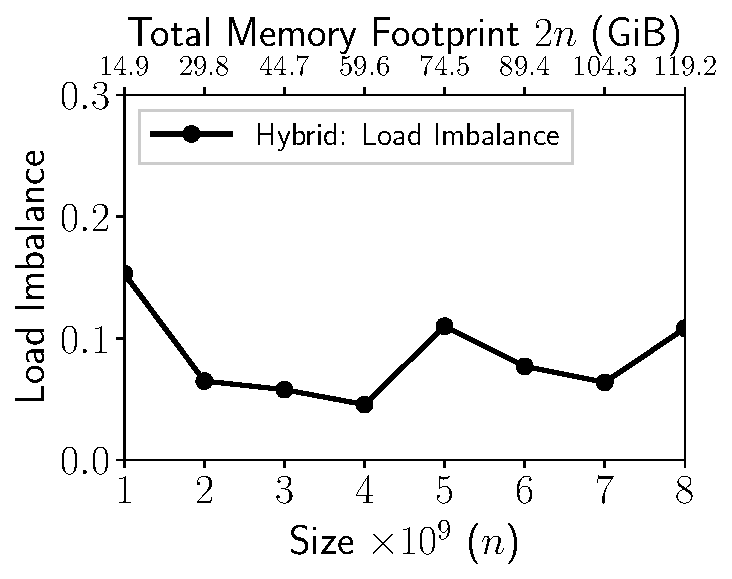
\includegraphics[height = 0.27\textwidth, width=0.30\textwidth, trim={0.2cm 0.2cm 0.2cm 0.2cm}]{figures/size_vs_load_imbalance_multiway.pdf}	
}
    \caption{The load imbalance of the hybrid algorithms in Figure 2.}
   \label{fig:scan_results}
\end{figure}

\end{block} 
\begin{description}[font=$\bullet$~\normalfont\scshape\color{red!50!black}]
\item We find that the hybrid model achieves a speedup over both the CPU-Only and GPU-Only times for the batched predecessor search and multiway merging $n$. 
\item However, the overheads associated with the hybrid algorithm for the scan result in a slowdown. With emerging technologies such as PCIe v4 the scan may see
  a speedup as we can assign more work to the GPU.
\end{description}


\begin{block}{Future Work}

\begin{description}[font=$\bullet$~\normalfont\scshape\color{red!50!black}]
%\item Investigating whether compression schemes or other memory transfer optimizations can alleviate some of the bottlenecks, despite the computational overhead.
\item The study of other fundamental operations that have not been considered for GPU acceleration.
\end{description}

\end{block}

%\begin{block}{Acknowledgements}
%This material is based upon work supported by the National Science Foundation under Grant OAC-1849559.
%\end{block}

\end{column}

\separatorcolumn
\end{columns}
\end{frame}

\end{document}
